% Options for packages loaded elsewhere
% Options for packages loaded elsewhere
\PassOptionsToPackage{unicode}{hyperref}
\PassOptionsToPackage{hyphens}{url}
\PassOptionsToPackage{dvipsnames,svgnames,x11names}{xcolor}
%
\documentclass[
  letterpaper,
  DIV=11,
  numbers=noendperiod]{scrartcl}
\usepackage{xcolor}
\usepackage{amsmath,amssymb}
\setcounter{secnumdepth}{-\maxdimen} % remove section numbering
\usepackage{iftex}
\ifPDFTeX
  \usepackage[T1]{fontenc}
  \usepackage[utf8]{inputenc}
  \usepackage{textcomp} % provide euro and other symbols
\else % if luatex or xetex
  \usepackage{unicode-math} % this also loads fontspec
  \defaultfontfeatures{Scale=MatchLowercase}
  \defaultfontfeatures[\rmfamily]{Ligatures=TeX,Scale=1}
\fi
\usepackage{lmodern}
\ifPDFTeX\else
  % xetex/luatex font selection
\fi
% Use upquote if available, for straight quotes in verbatim environments
\IfFileExists{upquote.sty}{\usepackage{upquote}}{}
\IfFileExists{microtype.sty}{% use microtype if available
  \usepackage[]{microtype}
  \UseMicrotypeSet[protrusion]{basicmath} % disable protrusion for tt fonts
}{}
\makeatletter
\@ifundefined{KOMAClassName}{% if non-KOMA class
  \IfFileExists{parskip.sty}{%
    \usepackage{parskip}
  }{% else
    \setlength{\parindent}{0pt}
    \setlength{\parskip}{6pt plus 2pt minus 1pt}}
}{% if KOMA class
  \KOMAoptions{parskip=half}}
\makeatother
% Make \paragraph and \subparagraph free-standing
\makeatletter
\ifx\paragraph\undefined\else
  \let\oldparagraph\paragraph
  \renewcommand{\paragraph}{
    \@ifstar
      \xxxParagraphStar
      \xxxParagraphNoStar
  }
  \newcommand{\xxxParagraphStar}[1]{\oldparagraph*{#1}\mbox{}}
  \newcommand{\xxxParagraphNoStar}[1]{\oldparagraph{#1}\mbox{}}
\fi
\ifx\subparagraph\undefined\else
  \let\oldsubparagraph\subparagraph
  \renewcommand{\subparagraph}{
    \@ifstar
      \xxxSubParagraphStar
      \xxxSubParagraphNoStar
  }
  \newcommand{\xxxSubParagraphStar}[1]{\oldsubparagraph*{#1}\mbox{}}
  \newcommand{\xxxSubParagraphNoStar}[1]{\oldsubparagraph{#1}\mbox{}}
\fi
\makeatother

\usepackage{color}
\usepackage{fancyvrb}
\newcommand{\VerbBar}{|}
\newcommand{\VERB}{\Verb[commandchars=\\\{\}]}
\DefineVerbatimEnvironment{Highlighting}{Verbatim}{commandchars=\\\{\}}
% Add ',fontsize=\small' for more characters per line
\usepackage{framed}
\definecolor{shadecolor}{RGB}{241,243,245}
\newenvironment{Shaded}{\begin{snugshade}}{\end{snugshade}}
\newcommand{\AlertTok}[1]{\textcolor[rgb]{0.68,0.00,0.00}{#1}}
\newcommand{\AnnotationTok}[1]{\textcolor[rgb]{0.37,0.37,0.37}{#1}}
\newcommand{\AttributeTok}[1]{\textcolor[rgb]{0.40,0.45,0.13}{#1}}
\newcommand{\BaseNTok}[1]{\textcolor[rgb]{0.68,0.00,0.00}{#1}}
\newcommand{\BuiltInTok}[1]{\textcolor[rgb]{0.00,0.23,0.31}{#1}}
\newcommand{\CharTok}[1]{\textcolor[rgb]{0.13,0.47,0.30}{#1}}
\newcommand{\CommentTok}[1]{\textcolor[rgb]{0.37,0.37,0.37}{#1}}
\newcommand{\CommentVarTok}[1]{\textcolor[rgb]{0.37,0.37,0.37}{\textit{#1}}}
\newcommand{\ConstantTok}[1]{\textcolor[rgb]{0.56,0.35,0.01}{#1}}
\newcommand{\ControlFlowTok}[1]{\textcolor[rgb]{0.00,0.23,0.31}{\textbf{#1}}}
\newcommand{\DataTypeTok}[1]{\textcolor[rgb]{0.68,0.00,0.00}{#1}}
\newcommand{\DecValTok}[1]{\textcolor[rgb]{0.68,0.00,0.00}{#1}}
\newcommand{\DocumentationTok}[1]{\textcolor[rgb]{0.37,0.37,0.37}{\textit{#1}}}
\newcommand{\ErrorTok}[1]{\textcolor[rgb]{0.68,0.00,0.00}{#1}}
\newcommand{\ExtensionTok}[1]{\textcolor[rgb]{0.00,0.23,0.31}{#1}}
\newcommand{\FloatTok}[1]{\textcolor[rgb]{0.68,0.00,0.00}{#1}}
\newcommand{\FunctionTok}[1]{\textcolor[rgb]{0.28,0.35,0.67}{#1}}
\newcommand{\ImportTok}[1]{\textcolor[rgb]{0.00,0.46,0.62}{#1}}
\newcommand{\InformationTok}[1]{\textcolor[rgb]{0.37,0.37,0.37}{#1}}
\newcommand{\KeywordTok}[1]{\textcolor[rgb]{0.00,0.23,0.31}{\textbf{#1}}}
\newcommand{\NormalTok}[1]{\textcolor[rgb]{0.00,0.23,0.31}{#1}}
\newcommand{\OperatorTok}[1]{\textcolor[rgb]{0.37,0.37,0.37}{#1}}
\newcommand{\OtherTok}[1]{\textcolor[rgb]{0.00,0.23,0.31}{#1}}
\newcommand{\PreprocessorTok}[1]{\textcolor[rgb]{0.68,0.00,0.00}{#1}}
\newcommand{\RegionMarkerTok}[1]{\textcolor[rgb]{0.00,0.23,0.31}{#1}}
\newcommand{\SpecialCharTok}[1]{\textcolor[rgb]{0.37,0.37,0.37}{#1}}
\newcommand{\SpecialStringTok}[1]{\textcolor[rgb]{0.13,0.47,0.30}{#1}}
\newcommand{\StringTok}[1]{\textcolor[rgb]{0.13,0.47,0.30}{#1}}
\newcommand{\VariableTok}[1]{\textcolor[rgb]{0.07,0.07,0.07}{#1}}
\newcommand{\VerbatimStringTok}[1]{\textcolor[rgb]{0.13,0.47,0.30}{#1}}
\newcommand{\WarningTok}[1]{\textcolor[rgb]{0.37,0.37,0.37}{\textit{#1}}}

\usepackage{longtable,booktabs,array}
\usepackage{calc} % for calculating minipage widths
% Correct order of tables after \paragraph or \subparagraph
\usepackage{etoolbox}
\makeatletter
\patchcmd\longtable{\par}{\if@noskipsec\mbox{}\fi\par}{}{}
\makeatother
% Allow footnotes in longtable head/foot
\IfFileExists{footnotehyper.sty}{\usepackage{footnotehyper}}{\usepackage{footnote}}
\makesavenoteenv{longtable}
\usepackage{graphicx}
\makeatletter
\newsavebox\pandoc@box
\newcommand*\pandocbounded[1]{% scales image to fit in text height/width
  \sbox\pandoc@box{#1}%
  \Gscale@div\@tempa{\textheight}{\dimexpr\ht\pandoc@box+\dp\pandoc@box\relax}%
  \Gscale@div\@tempb{\linewidth}{\wd\pandoc@box}%
  \ifdim\@tempb\p@<\@tempa\p@\let\@tempa\@tempb\fi% select the smaller of both
  \ifdim\@tempa\p@<\p@\scalebox{\@tempa}{\usebox\pandoc@box}%
  \else\usebox{\pandoc@box}%
  \fi%
}
% Set default figure placement to htbp
\def\fps@figure{htbp}
\makeatother





\setlength{\emergencystretch}{3em} % prevent overfull lines

\providecommand{\tightlist}{%
  \setlength{\itemsep}{0pt}\setlength{\parskip}{0pt}}



 


\KOMAoption{captions}{tableheading}
\makeatletter
\@ifpackageloaded{caption}{}{\usepackage{caption}}
\AtBeginDocument{%
\ifdefined\contentsname
  \renewcommand*\contentsname{Table of contents}
\else
  \newcommand\contentsname{Table of contents}
\fi
\ifdefined\listfigurename
  \renewcommand*\listfigurename{List of Figures}
\else
  \newcommand\listfigurename{List of Figures}
\fi
\ifdefined\listtablename
  \renewcommand*\listtablename{List of Tables}
\else
  \newcommand\listtablename{List of Tables}
\fi
\ifdefined\figurename
  \renewcommand*\figurename{Figure}
\else
  \newcommand\figurename{Figure}
\fi
\ifdefined\tablename
  \renewcommand*\tablename{Table}
\else
  \newcommand\tablename{Table}
\fi
}
\@ifpackageloaded{float}{}{\usepackage{float}}
\floatstyle{ruled}
\@ifundefined{c@chapter}{\newfloat{codelisting}{h}{lop}}{\newfloat{codelisting}{h}{lop}[chapter]}
\floatname{codelisting}{Listing}
\newcommand*\listoflistings{\listof{codelisting}{List of Listings}}
\makeatother
\makeatletter
\makeatother
\makeatletter
\@ifpackageloaded{caption}{}{\usepackage{caption}}
\@ifpackageloaded{subcaption}{}{\usepackage{subcaption}}
\makeatother
\usepackage{bookmark}
\IfFileExists{xurl.sty}{\usepackage{xurl}}{} % add URL line breaks if available
\urlstyle{same}
\hypersetup{
  colorlinks=true,
  linkcolor={blue},
  filecolor={Maroon},
  citecolor={Blue},
  urlcolor={Blue},
  pdfcreator={LaTeX via pandoc}}


\author{}
\date{}
\begin{document}


`Opponent', `Is\_Home', `Result', `Goals', `Opponent\_Goals',
`Possession', `Shots', `Shots\_On\_Target', `Passes\_Completed',
`Pass\_Accuracy', `Corners', `Crosses', `Fouls', `Offsides',
`Opponent\_Possession', `Opponent\_Shots',
`Opponent\_Shots\_On\_Target', `Opponent\_Passes\_Completed',
`Opponent\_Pass\_Accuracy', `Opponent\_Corners', `Opponent\_Crosses',
`Opponent\_Fouls', `Opponent\_Offsides', `Shot\_Efficiency', `Season',
`Month', `Day\_of\_Week', `Last5\_Avg\_Goals', `Last5\_Win\_Rate',
`club\_name', `Date\_day', `Date\_month', `Date\_year', `Date\_weekday',
`Date\_quarter', `Date\_hour', `Date\_minute', `Date\_second'

\begin{Shaded}
\begin{Highlighting}[]
\ImportTok{import}\NormalTok{ requests}
\ImportTok{import}\NormalTok{ zipfile}
\ImportTok{import}\NormalTok{ io}
\ImportTok{import}\NormalTok{ pandas }\ImportTok{as}\NormalTok{ pd}
\ImportTok{import}\NormalTok{ seaborn }\ImportTok{as}\NormalTok{ sns}
\ImportTok{import}\NormalTok{ matplotlib.pyplot }\ImportTok{as}\NormalTok{ plt}
\ImportTok{from}\NormalTok{ plotnine }\ImportTok{import} \OperatorTok{*}
\ImportTok{from}\NormalTok{ sklearn.preprocessing }\ImportTok{import}\NormalTok{ LabelEncoder}
\ImportTok{import}\NormalTok{ plotly.express }\ImportTok{as}\NormalTok{ px}

\CommentTok{\# URL del dataset en Kaggle (funcionando con requests en tu caso)}
\NormalTok{url }\OperatorTok{=} \StringTok{"https://www.kaggle.com/api/v1/datasets/download/ensarakbas/premier{-}league{-}top{-}6{-}teams{-}match{-}statistics"}

\CommentTok{\# Descargar el zip}
\NormalTok{response }\OperatorTok{=}\NormalTok{ requests.get(url, allow\_redirects}\OperatorTok{=}\VariableTok{True}\NormalTok{)}

\ControlFlowTok{if}\NormalTok{ response.status\_code }\OperatorTok{==} \DecValTok{200}\NormalTok{:}
    \BuiltInTok{print}\NormalTok{(}\StringTok{"download completed "}\NormalTok{)}

    \CommentTok{\# Abrir el zip desde memoria}
    \ControlFlowTok{with}\NormalTok{ zipfile.ZipFile(io.BytesIO(response.content)) }\ImportTok{as}\NormalTok{ zip\_file:}
        \BuiltInTok{print}\NormalTok{(}\StringTok{"files in zip:"}\NormalTok{, zip\_file.namelist())}

        \CommentTok{\# Filtrar solo archivos CSV}
\NormalTok{        csv\_files }\OperatorTok{=}\NormalTok{ [name }\ControlFlowTok{for}\NormalTok{ name }\KeywordTok{in}\NormalTok{ zip\_file.namelist() }\ControlFlowTok{if}\NormalTok{ name.endswith(}\StringTok{".csv"}\NormalTok{)]}

        \CommentTok{\# Leer todos los CSVs en una lista de DataFrames}
\NormalTok{        dfs }\OperatorTok{=}\NormalTok{ []}
        \ControlFlowTok{for}\NormalTok{ name }\KeywordTok{in}\NormalTok{ csv\_files:}
            \BuiltInTok{print}\NormalTok{(}\SpecialStringTok{f"reading csv }\SpecialCharTok{\{}\NormalTok{name}\SpecialCharTok{\}}\SpecialStringTok{..."}\NormalTok{)}
\NormalTok{            df\_temp }\OperatorTok{=}\NormalTok{ pd.read\_csv(zip\_file.}\BuiltInTok{open}\NormalTok{(name))}
\NormalTok{            df\_temp[}\StringTok{"origen\_csv"}\NormalTok{] }\OperatorTok{=}\NormalTok{ name  }\CommentTok{\# opcional: para saber de qué archivo vino}
\NormalTok{            dfs.append(df\_temp)}

        \CommentTok{\# Concatenar todo en un único DataFrame}
\NormalTok{        df\_final }\OperatorTok{=}\NormalTok{ pd.concat(dfs, ignore\_index}\OperatorTok{=}\VariableTok{True}\NormalTok{)}

\NormalTok{        aliquota }\OperatorTok{=}\NormalTok{ df\_final.sample(n}\OperatorTok{=}\DecValTok{50}\NormalTok{, random\_state}\OperatorTok{=}\DecValTok{32}\NormalTok{)}

        \CommentTok{\# Guardar la alícuota en un CSV separado}
\NormalTok{        aliquota.to\_csv(}\StringTok{"aliquota\_test.csv"}\NormalTok{, index}\OperatorTok{=}\VariableTok{False}\NormalTok{)}

        \CommentTok{\# Eliminar las filas seleccionadas del dataset original para entrenamiento}
\NormalTok{        df\_final }\OperatorTok{=}\NormalTok{ df\_final.drop(aliquota.index).reset\_index(drop}\OperatorTok{=}\VariableTok{True}\NormalTok{)}

        \BuiltInTok{print}\NormalTok{(}\StringTok{"df merged ready"}\NormalTok{)}
        \BuiltInTok{print}\NormalTok{(}\StringTok{"final shape:"}\NormalTok{, df\_final.shape)}
\NormalTok{        df\_final.head(}\DecValTok{5}\NormalTok{)}
\ControlFlowTok{else}\NormalTok{:}
    \BuiltInTok{print}\NormalTok{(}\StringTok{"download failed:"}\NormalTok{, response.status\_code)}

\end{Highlighting}
\end{Shaded}

\begin{verbatim}
download completed 
files in zip: ['Arsenal.csv', 'Chelsea.csv', 'Liverpool.csv', 'Manchester City.csv', 'Manchester United.csv', 'Tottenham.csv']
reading csv Arsenal.csv...
reading csv Chelsea.csv...
reading csv Liverpool.csv...
reading csv Manchester City.csv...
reading csv Manchester United.csv...
reading csv Tottenham.csv...
df merged ready
final shape: (4144, 31)
\end{verbatim}

\begin{Shaded}
\begin{Highlighting}[]

\NormalTok{df\_final[}\StringTok{\textquotesingle{}club\_name\textquotesingle{}}\NormalTok{] }\OperatorTok{=}\NormalTok{ df\_final[}\StringTok{\textquotesingle{}origen\_csv\textquotesingle{}}\NormalTok{].}\BuiltInTok{str}\NormalTok{.replace(}\StringTok{\textquotesingle{}.csv\textquotesingle{}}\NormalTok{, }\StringTok{\textquotesingle{}\textquotesingle{}}\NormalTok{, regex}\OperatorTok{=}\VariableTok{False}\NormalTok{)}

\NormalTok{df\_final }\OperatorTok{=}\NormalTok{ df\_final.drop(columns}\OperatorTok{=}\NormalTok{[}\StringTok{\textquotesingle{}origen\_csv\textquotesingle{}}\NormalTok{])}

\end{Highlighting}
\end{Shaded}

\begin{Shaded}
\begin{Highlighting}[]
\NormalTok{df\_final.head(}\DecValTok{5}\NormalTok{)}
\end{Highlighting}
\end{Shaded}

\begin{longtable}[]{@{}llllllllllllllllllllllllllllllll@{}}
\toprule\noalign{}
& Date & Opponent & Is\_Home & Result & Goals & Opponent\_Goals &
Possession & Shots & Shots\_On\_Target & Passes\_Completed &
Pass\_Accuracy & Corners & Crosses & Fouls & Offsides &
Opponent\_Possession & Opponent\_Shots & Opponent\_Shots\_On\_Target &
Opponent\_Passes\_Completed & Opponent\_Pass\_Accuracy &
Opponent\_Corners & Opponent\_Crosses & Opponent\_Fouls &
Opponent\_Offsides & Shot\_Efficiency & Season & Month & Day\_of\_Week &
Last5\_Avg\_Goals & Last5\_Win\_Rate & club\_name \\
\midrule\noalign{}
\endhead
\bottomrule\noalign{}
\endlastfoot
0 & 2013-08-04 18:20:00 & Galatasaray & 1 & -1 & 1 & 2 & 55 & 12 & 5 &
425 & 80 & 4 & 2 & 12 & 2 & 45 & 12 & 6 & 399 & 81 & 5 & 3 & 15 & 2 &
0.416667 & 2013 & 8 & 7 & 1.000000 & 0.00 & Arsenal \\
1 & 2013-08-17 17:00:00 & Aston Villa & 1 & -1 & 1 & 3 & 64 & 15 & 4 &
457 & 87 & 4 & 4 & 15 & 3 & 36 & 10 & 5 & 216 & 71 & 3 & 2 & 19 & 1 &
0.266667 & 2013 & 8 & 6 & 1.000000 & 0.00 & Arsenal \\
2 & 2013-08-21 21:45:00 & Fenerbahçe & 0 & 1 & 3 & 0 & 60 & 13 & 7 & 451
& 84 & 6 & 2 & 14 & 0 & 40 & 6 & 2 & 350 & 79 & 5 & 2 & 15 & 1 &
0.538462 & 2013 & 8 & 3 & 1.666667 & 0.33 & Arsenal \\
3 & 2013-08-24 14:45:00 & Fulham & 0 & 1 & 3 & 1 & 54 & 19 & 9 & 496 &
87 & 8 & 9 & 9 & 0 & 46 & 16 & 7 & 421 & 87 & 1 & 1 & 10 & 3 & 0.473684
& 2013 & 8 & 6 & 2.000000 & 0.50 & Arsenal \\
4 & 2013-08-27 21:45:00 & Fenerbahçe & 1 & 1 & 2 & 0 & 65 & 14 & 6 & 460
& 86 & 2 & 4 & 16 & 2 & 35 & 6 & 4 & 350 & 79 & 3 & 4 & 16 & 1 &
0.428571 & 2013 & 8 & 2 & 2.000000 & 0.60 & Arsenal \\
\end{longtable}

\begin{Shaded}
\begin{Highlighting}[]
\NormalTok{df\_final.info()}
\end{Highlighting}
\end{Shaded}

\begin{verbatim}
<class 'pandas.core.frame.DataFrame'>
RangeIndex: 4144 entries, 0 to 4143
Data columns (total 31 columns):
 #   Column                     Non-Null Count  Dtype  
---  ------                     --------------  -----  
 0   Date                       4144 non-null   object 
 1   Opponent                   4144 non-null   object 
 2   Is_Home                    4144 non-null   int64  
 3   Result                     4144 non-null   int64  
 4   Goals                      4144 non-null   int64  
 5   Opponent_Goals             4144 non-null   int64  
 6   Possession                 4144 non-null   int64  
 7   Shots                      4144 non-null   int64  
 8   Shots_On_Target            4144 non-null   int64  
 9   Passes_Completed           4144 non-null   int64  
 10  Pass_Accuracy              4144 non-null   int64  
 11  Corners                    4144 non-null   int64  
 12  Crosses                    4144 non-null   int64  
 13  Fouls                      4144 non-null   int64  
 14  Offsides                   4144 non-null   int64  
 15  Opponent_Possession        4144 non-null   int64  
 16  Opponent_Shots             4144 non-null   int64  
 17  Opponent_Shots_On_Target   4144 non-null   int64  
 18  Opponent_Passes_Completed  4144 non-null   int64  
 19  Opponent_Pass_Accuracy     4144 non-null   int64  
 20  Opponent_Corners           4144 non-null   int64  
 21  Opponent_Crosses           4144 non-null   int64  
 22  Opponent_Fouls             4144 non-null   int64  
 23  Opponent_Offsides          4144 non-null   int64  
 24  Shot_Efficiency            4143 non-null   float64
 25  Season                     4144 non-null   int64  
 26  Month                      4144 non-null   int64  
 27  Day_of_Week                4144 non-null   int64  
 28  Last5_Avg_Goals            4144 non-null   float64
 29  Last5_Win_Rate             4144 non-null   float64
 30  club_name                  4144 non-null   object 
dtypes: float64(3), int64(25), object(3)
memory usage: 1003.8+ KB
\end{verbatim}

\begin{Shaded}
\begin{Highlighting}[]
\NormalTok{df\_final.describe()}
\end{Highlighting}
\end{Shaded}

\begin{longtable}[]{@{}lllllllllllllllllllllllllllll@{}}
\toprule\noalign{}
& Is\_Home & Result & Goals & Opponent\_Goals & Possession & Shots &
Shots\_On\_Target & Passes\_Completed & Pass\_Accuracy & Corners &
Crosses & Fouls & Offsides & Opponent\_Possession & Opponent\_Shots &
Opponent\_Shots\_On\_Target & Opponent\_Passes\_Completed &
Opponent\_Pass\_Accuracy & Opponent\_Corners & Opponent\_Crosses &
Opponent\_Fouls & Opponent\_Offsides & Shot\_Efficiency & Season & Month
& Day\_of\_Week & Last5\_Avg\_Goals & Last5\_Win\_Rate \\
\midrule\noalign{}
\endhead
\bottomrule\noalign{}
\endlastfoot
count & 4144.000000 & 4144.000000 & 4144.000000 & 4144.000000 &
4144.000000 & 4144.000000 & 4144.000000 & 4144.000000 & 4144.000000 &
4144.000000 & 4144.000000 & 4144.000000 & 4144.000000 & 4144.000000 &
4144.000000 & 4144.000000 & 4144.000000 & 4144.000000 & 4144.000000 &
4144.000000 & 4144.000000 & 4144.000000 & 4143.000000 & 4144.000000 &
4144.000000 & 4144.000000 & 4144.000000 & 4144.000000 \\
mean & 0.504344 & 0.349180 & 1.958253 & 1.075048 & 58.019788 & 15.143581
& 5.610763 & 477.937259 & 84.330116 & 5.976351 & 4.195946 & 10.751689 &
1.987693 & 41.958977 & 10.364624 & 3.624276 & 318.765444 & 77.222973 &
4.130309 & 3.383929 & 10.800193 & 2.073600 & 0.378714 & 2019.015685 &
6.627172 & 4.926400 & 1.957650 & 0.577667 \\
std & 0.500041 & 0.825279 & 1.486262 & 1.102918 & 10.907931 & 6.049829 &
2.835806 & 124.248427 & 5.029155 & 3.165393 & 2.671891 & 3.763318 &
1.650370 & 10.889002 & 4.895432 & 2.261880 & 116.718049 & 8.038196 &
2.626736 & 2.367827 & 3.731922 & 1.670444 & 0.147749 & 3.373806 &
3.818947 & 1.937507 & 0.733888 & 0.231944 \\
min & 0.000000 & -1.000000 & 0.000000 & 0.000000 & 0.000000 & 0.000000 &
0.000000 & 94.000000 & 49.000000 & 0.000000 & 0.000000 & 0.000000 &
0.000000 & 0.000000 & 0.000000 & 0.000000 & 71.000000 & 0.000000 &
0.000000 & 0.000000 & 0.000000 & 0.000000 & 0.000000 & 2011.000000 &
1.000000 & 1.000000 & 0.000000 & 0.000000 \\
25\% & 0.000000 & 0.000000 & 1.000000 & 0.000000 & 51.000000 & 11.000000
& 4.000000 & 393.000000 & 81.000000 & 4.000000 & 2.000000 & 8.000000 &
1.000000 & 34.000000 & 7.000000 & 2.000000 & 230.000000 & 72.000000 &
2.000000 & 2.000000 & 8.000000 & 1.000000 & 0.277778 & 2016.000000 &
3.000000 & 3.000000 & 1.400000 & 0.400000 \\
50\% & 1.000000 & 1.000000 & 2.000000 & 1.000000 & 59.000000 & 15.000000
& 5.000000 & 473.000000 & 85.000000 & 6.000000 & 4.000000 & 11.000000 &
2.000000 & 41.000000 & 10.000000 & 3.000000 & 304.000000 & 78.000000 &
4.000000 & 3.000000 & 11.000000 & 2.000000 & 0.368421 & 2019.000000 &
7.000000 & 6.000000 & 2.000000 & 0.600000 \\
75\% & 1.000000 & 1.000000 & 3.000000 & 2.000000 & 66.000000 & 19.000000
& 7.000000 & 559.000000 & 88.000000 & 8.000000 & 6.000000 & 13.000000 &
3.000000 & 49.000000 & 13.000000 & 5.000000 & 392.000000 & 83.000000 &
6.000000 & 5.000000 & 13.000000 & 3.000000 & 0.466667 & 2022.000000 &
10.000000 & 7.000000 & 2.400000 & 0.800000 \\
max & 1.000000 & 1.000000 & 9.000000 & 7.000000 & 84.000000 & 58.000000
& 20.000000 & 979.000000 & 96.000000 & 20.000000 & 24.000000 & 25.000000
& 12.000000 & 80.000000 & 36.000000 & 16.000000 & 902.000000 & 95.000000
& 17.000000 & 16.000000 & 27.000000 & 11.000000 & 1.000000 & 2025.000000
& 12.000000 & 7.000000 & 6.000000 & 1.000000 \\
\end{longtable}

\begin{Shaded}
\begin{Highlighting}[]
\NormalTok{dfnull }\OperatorTok{=}\NormalTok{ df\_final.isnull().}\BuiltInTok{sum}\NormalTok{().reset\_index()}
\NormalTok{dfnull.columns }\OperatorTok{=}\NormalTok{ [}\StringTok{\textquotesingle{}column\textquotesingle{}}\NormalTok{, }\StringTok{\textquotesingle{}nulls\textquotesingle{}}\NormalTok{]}
\NormalTok{dfnull}\OperatorTok{=}\NormalTok{dfnull.query(}\StringTok{" nulls \textgreater{} 0"}\NormalTok{)}
\NormalTok{dfnull[}\StringTok{\textquotesingle{}mean\textquotesingle{}}\NormalTok{]}\OperatorTok{=}\NormalTok{dfnull[}\StringTok{\textquotesingle{}nulls\textquotesingle{}}\NormalTok{].mean()}

\end{Highlighting}
\end{Shaded}

\begin{Shaded}
\begin{Highlighting}[]
\NormalTok{plt.figure(figsize}\OperatorTok{=}\NormalTok{(}\DecValTok{12}\NormalTok{, }\DecValTok{6}\NormalTok{))}
\NormalTok{sns.heatmap(dfnull[[}\StringTok{\textquotesingle{}nulls\textquotesingle{}}\NormalTok{]].set\_index(dfnull[}\StringTok{\textquotesingle{}column\textquotesingle{}}\NormalTok{]), annot}\OperatorTok{=}\VariableTok{True}\NormalTok{, cmap}\OperatorTok{=}\StringTok{"Reds"}\NormalTok{,fmt}\OperatorTok{=}\StringTok{"d"}\NormalTok{)}
\NormalTok{plt.show()}
\end{Highlighting}
\end{Shaded}

\pandocbounded{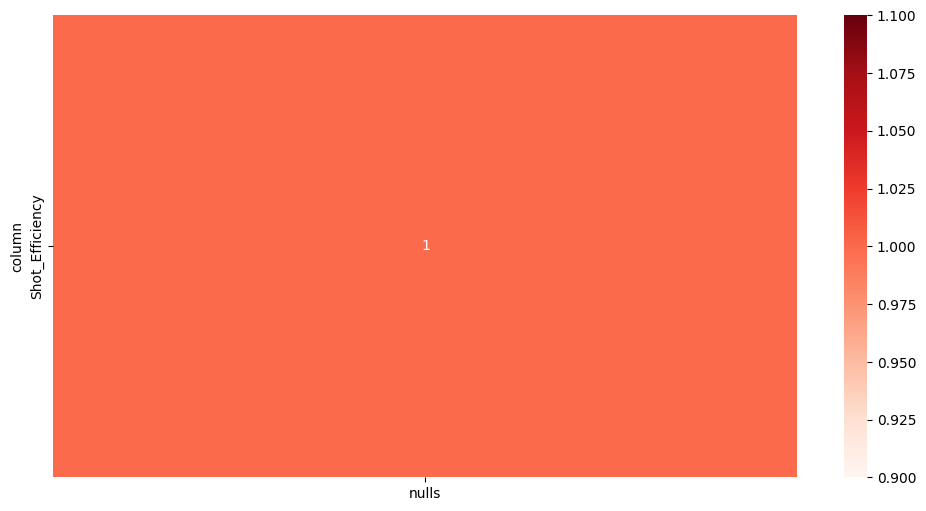
\includegraphics[keepaspectratio]{premier_league_files/figure-pdf/cell-8-output-1.png}}

\begin{Shaded}
\begin{Highlighting}[]
\NormalTok{df\_final[}\StringTok{\textquotesingle{}Shot\_Efficiency\textquotesingle{}}\NormalTok{]}\OperatorTok{=}\NormalTok{df\_final[}\StringTok{\textquotesingle{}Shot\_Efficiency\textquotesingle{}}\NormalTok{].fillna(df\_final[}\StringTok{\textquotesingle{}Shot\_Efficiency\textquotesingle{}}\NormalTok{].mean())}
\end{Highlighting}
\end{Shaded}

\begin{Shaded}
\begin{Highlighting}[]
\NormalTok{df\_final[}\StringTok{\textquotesingle{}Shot\_Efficiency\textquotesingle{}}\NormalTok{].isnull().}\BuiltInTok{sum}\NormalTok{()}
\end{Highlighting}
\end{Shaded}

\begin{verbatim}
np.int64(0)
\end{verbatim}

\begin{Shaded}
\begin{Highlighting}[]
\KeywordTok{def}\NormalTok{ preprocess\_dates(df):}
    \CommentTok{"""}
\CommentTok{     transforma columnas de fechas en columnas numéricas.}
\CommentTok{    }
\CommentTok{    Args:}
\CommentTok{        df (pd.DataFrame): DataFrame original}
\CommentTok{    }
\CommentTok{    Returns:}
\CommentTok{        pd.DataFrame: DataFrame con columnas de fecha convertidas a componentes numéricos}
\CommentTok{    """}
    
    \CommentTok{\# Columnas de fechas a transformar}
\NormalTok{    dates\_encode }\OperatorTok{=}\NormalTok{ [}\StringTok{\textquotesingle{}Date\textquotesingle{}}\NormalTok{]}
    
    \ControlFlowTok{for}\NormalTok{ col }\KeywordTok{in}\NormalTok{ dates\_encode:}
        \ControlFlowTok{if}\NormalTok{ col }\KeywordTok{in}\NormalTok{ df.columns:}
            \CommentTok{\# Convertir a datetime (auto detecta formato tipo 2013{-}08{-}04 18:20:00)}
\NormalTok{            df[col] }\OperatorTok{=}\NormalTok{ pd.to\_datetime(df[col], errors}\OperatorTok{=}\StringTok{\textquotesingle{}coerce\textquotesingle{}}\NormalTok{)}
            
            \CommentTok{\# Extraer componentes de fecha}
\NormalTok{            df[col }\OperatorTok{+} \StringTok{\textquotesingle{}\_day\textquotesingle{}}\NormalTok{]      }\OperatorTok{=}\NormalTok{ df[col].dt.day.fillna(}\DecValTok{0}\NormalTok{).astype(}\StringTok{\textquotesingle{}int32\textquotesingle{}}\NormalTok{)}
\NormalTok{            df[col }\OperatorTok{+} \StringTok{\textquotesingle{}\_month\textquotesingle{}}\NormalTok{]    }\OperatorTok{=}\NormalTok{ df[col].dt.month.fillna(}\DecValTok{0}\NormalTok{).astype(}\StringTok{\textquotesingle{}int32\textquotesingle{}}\NormalTok{)}
\NormalTok{            df[col }\OperatorTok{+} \StringTok{\textquotesingle{}\_year\textquotesingle{}}\NormalTok{]     }\OperatorTok{=}\NormalTok{ df[col].dt.year.fillna(}\DecValTok{0}\NormalTok{).astype(}\StringTok{\textquotesingle{}int32\textquotesingle{}}\NormalTok{)}
\NormalTok{            df[col }\OperatorTok{+} \StringTok{\textquotesingle{}\_weekday\textquotesingle{}}\NormalTok{]  }\OperatorTok{=}\NormalTok{ df[col].dt.weekday.fillna(}\DecValTok{0}\NormalTok{).astype(}\StringTok{\textquotesingle{}int32\textquotesingle{}}\NormalTok{)}
\NormalTok{            df[col }\OperatorTok{+} \StringTok{\textquotesingle{}\_quarter\textquotesingle{}}\NormalTok{]  }\OperatorTok{=}\NormalTok{ df[col].dt.quarter.fillna(}\DecValTok{0}\NormalTok{).astype(}\StringTok{\textquotesingle{}int32\textquotesingle{}}\NormalTok{)}
            
            \CommentTok{\# Extraer componentes de tiempo (por si querés usarlos también)}
\NormalTok{            df[col }\OperatorTok{+} \StringTok{\textquotesingle{}\_hour\textquotesingle{}}\NormalTok{]     }\OperatorTok{=}\NormalTok{ df[col].dt.hour.fillna(}\DecValTok{0}\NormalTok{).astype(}\StringTok{\textquotesingle{}int32\textquotesingle{}}\NormalTok{)}
\NormalTok{            df[col }\OperatorTok{+} \StringTok{\textquotesingle{}\_minute\textquotesingle{}}\NormalTok{]   }\OperatorTok{=}\NormalTok{ df[col].dt.minute.fillna(}\DecValTok{0}\NormalTok{).astype(}\StringTok{\textquotesingle{}int32\textquotesingle{}}\NormalTok{)}
\NormalTok{            df[col }\OperatorTok{+} \StringTok{\textquotesingle{}\_second\textquotesingle{}}\NormalTok{]   }\OperatorTok{=}\NormalTok{ df[col].dt.second.fillna(}\DecValTok{0}\NormalTok{).astype(}\StringTok{\textquotesingle{}int32\textquotesingle{}}\NormalTok{)}
    
    \CommentTok{\# Eliminar las columnas de fecha originales}
\NormalTok{    df.drop(columns}\OperatorTok{=}\NormalTok{[c }\ControlFlowTok{for}\NormalTok{ c }\KeywordTok{in}\NormalTok{ dates\_encode }\ControlFlowTok{if}\NormalTok{ c }\KeywordTok{in}\NormalTok{ df.columns], inplace}\OperatorTok{=}\VariableTok{True}\NormalTok{)}
    
    \ControlFlowTok{return}\NormalTok{ df}
\end{Highlighting}
\end{Shaded}

\begin{Shaded}
\begin{Highlighting}[]
\NormalTok{df\_final}\OperatorTok{=}\NormalTok{preprocess\_dates(df\_final)}
\NormalTok{df\_final.head(}\DecValTok{5}\NormalTok{)}
\end{Highlighting}
\end{Shaded}

\begin{longtable}[]{@{}llllllllllllllllllllll@{}}
\toprule\noalign{}
& Opponent & Is\_Home & Result & Goals & Opponent\_Goals & Possession &
Shots & Shots\_On\_Target & Passes\_Completed & Pass\_Accuracy & ... &
Last5\_Win\_Rate & club\_name & Date\_day & Date\_month & Date\_year &
Date\_weekday & Date\_quarter & Date\_hour & Date\_minute &
Date\_second \\
\midrule\noalign{}
\endhead
\bottomrule\noalign{}
\endlastfoot
0 & Galatasaray & 1 & -1 & 1 & 2 & 55 & 12 & 5 & 425 & 80 & ... & 0.00 &
Arsenal & 4 & 8 & 2013 & 6 & 3 & 18 & 20 & 0 \\
1 & Aston Villa & 1 & -1 & 1 & 3 & 64 & 15 & 4 & 457 & 87 & ... & 0.00 &
Arsenal & 17 & 8 & 2013 & 5 & 3 & 17 & 0 & 0 \\
2 & Fenerbahçe & 0 & 1 & 3 & 0 & 60 & 13 & 7 & 451 & 84 & ... & 0.33 &
Arsenal & 21 & 8 & 2013 & 2 & 3 & 21 & 45 & 0 \\
3 & Fulham & 0 & 1 & 3 & 1 & 54 & 19 & 9 & 496 & 87 & ... & 0.50 &
Arsenal & 24 & 8 & 2013 & 5 & 3 & 14 & 45 & 0 \\
4 & Fenerbahçe & 1 & 1 & 2 & 0 & 65 & 14 & 6 & 460 & 86 & ... & 0.60 &
Arsenal & 27 & 8 & 2013 & 1 & 3 & 21 & 45 & 0 \\
\end{longtable}

\begin{Shaded}
\begin{Highlighting}[]
\NormalTok{df\_final[}\StringTok{\textquotesingle{}Opponent\textquotesingle{}}\NormalTok{].drop\_duplicates().shape}
\end{Highlighting}
\end{Shaded}

\begin{verbatim}
(478,)
\end{verbatim}

\begin{Shaded}
\begin{Highlighting}[]

\NormalTok{plt.figure(figsize}\OperatorTok{=}\NormalTok{(}\DecValTok{10}\NormalTok{, }\DecValTok{8}\NormalTok{))}
\NormalTok{sns.scatterplot(x}\OperatorTok{=}\StringTok{\textquotesingle{}Opponent\_Possession\textquotesingle{}}\NormalTok{, y}\OperatorTok{=}\StringTok{\textquotesingle{}Passes\_Completed\textquotesingle{}}\NormalTok{, data}\OperatorTok{=}\NormalTok{df\_final, hue}\OperatorTok{=}\StringTok{\textquotesingle{}club\_name\textquotesingle{}}\NormalTok{,palette}\OperatorTok{=}\StringTok{\textquotesingle{}Set1\textquotesingle{}}\NormalTok{)}
\NormalTok{plt.show()}
\end{Highlighting}
\end{Shaded}

\pandocbounded{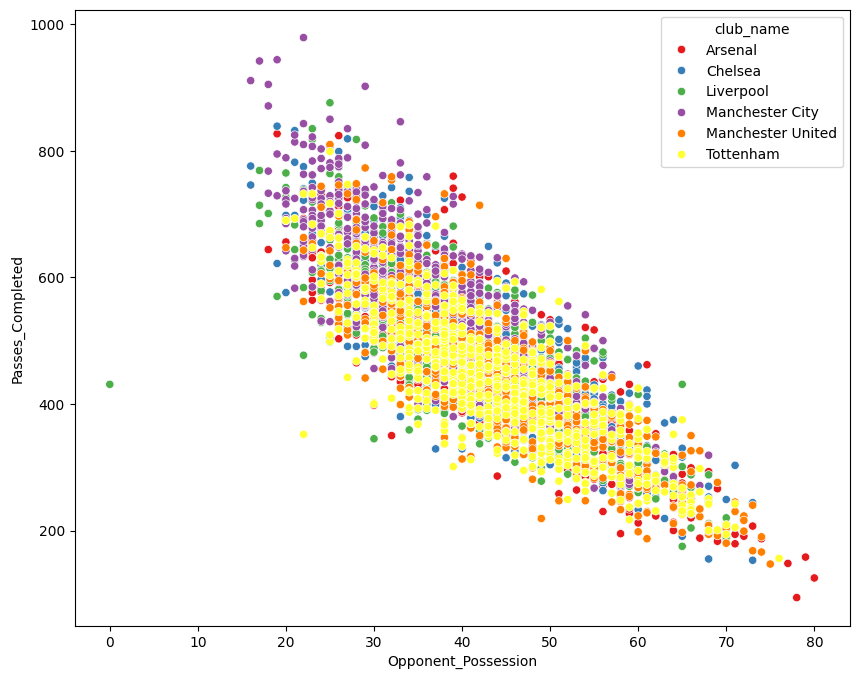
\includegraphics[keepaspectratio]{premier_league_files/figure-pdf/cell-14-output-1.png}}

\begin{Shaded}
\begin{Highlighting}[]

\NormalTok{plt.figure(figsize}\OperatorTok{=}\NormalTok{(}\DecValTok{10}\NormalTok{, }\DecValTok{8}\NormalTok{))}
\NormalTok{sns.barplot(x}\OperatorTok{=}\StringTok{\textquotesingle{}club\_name\textquotesingle{}}\NormalTok{, y}\OperatorTok{=}\StringTok{\textquotesingle{}Passes\_Completed\textquotesingle{}}\NormalTok{, data}\OperatorTok{=}\NormalTok{df\_final, hue}\OperatorTok{=}\StringTok{\textquotesingle{}Is\_Home\textquotesingle{}}\NormalTok{,palette}\OperatorTok{=}\StringTok{\textquotesingle{}Set1\textquotesingle{}}\NormalTok{)}
\NormalTok{plt.show()}
\end{Highlighting}
\end{Shaded}

\pandocbounded{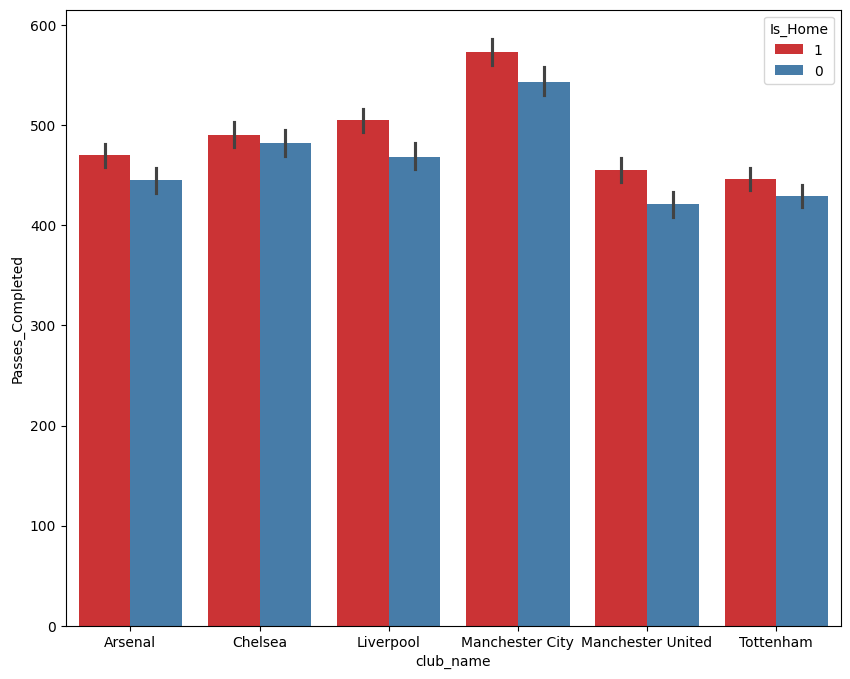
\includegraphics[keepaspectratio]{premier_league_files/figure-pdf/cell-15-output-1.png}}

\begin{Shaded}
\begin{Highlighting}[]
\NormalTok{df\_final[}\StringTok{\textquotesingle{}Is\_Home\textquotesingle{}}\NormalTok{]}\OperatorTok{=}\NormalTok{df\_final[}\StringTok{\textquotesingle{}Is\_Home\textquotesingle{}}\NormalTok{].astype(}\BuiltInTok{str}\NormalTok{)}
\end{Highlighting}
\end{Shaded}

\begin{Shaded}
\begin{Highlighting}[]

\NormalTok{plt.figure(figsize}\OperatorTok{=}\NormalTok{(}\DecValTok{10}\NormalTok{, }\DecValTok{8}\NormalTok{))}
\NormalTok{sns.barplot(x}\OperatorTok{=}\StringTok{\textquotesingle{}club\_name\textquotesingle{}}\NormalTok{, y}\OperatorTok{=}\StringTok{\textquotesingle{}Goals\textquotesingle{}}\NormalTok{,hue}\OperatorTok{=}\StringTok{\textquotesingle{}Is\_Home\textquotesingle{}}\NormalTok{, data}\OperatorTok{=}\NormalTok{df\_final)}
\NormalTok{plt.show()}
\end{Highlighting}
\end{Shaded}

\pandocbounded{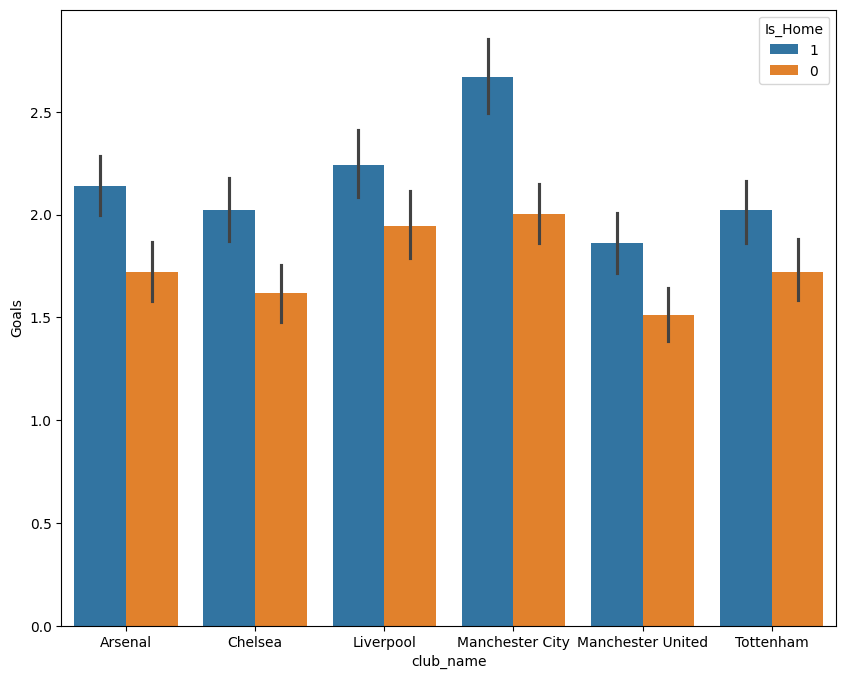
\includegraphics[keepaspectratio]{premier_league_files/figure-pdf/cell-17-output-1.png}}

\begin{Shaded}
\begin{Highlighting}[]

\NormalTok{plt.figure(figsize}\OperatorTok{=}\NormalTok{(}\DecValTok{10}\NormalTok{, }\DecValTok{8}\NormalTok{))}
\NormalTok{sns.histplot(x}\OperatorTok{=}\StringTok{\textquotesingle{}Result\textquotesingle{}}\NormalTok{ ,data}\OperatorTok{=}\NormalTok{df\_final, hue}\OperatorTok{=}\StringTok{\textquotesingle{}club\_name\textquotesingle{}}\NormalTok{,palette}\OperatorTok{=}\StringTok{\textquotesingle{}Set1\textquotesingle{}}\NormalTok{,multiple}\OperatorTok{=}\StringTok{"dodge"}\NormalTok{, )}
\NormalTok{plt.show()}
\end{Highlighting}
\end{Shaded}

\pandocbounded{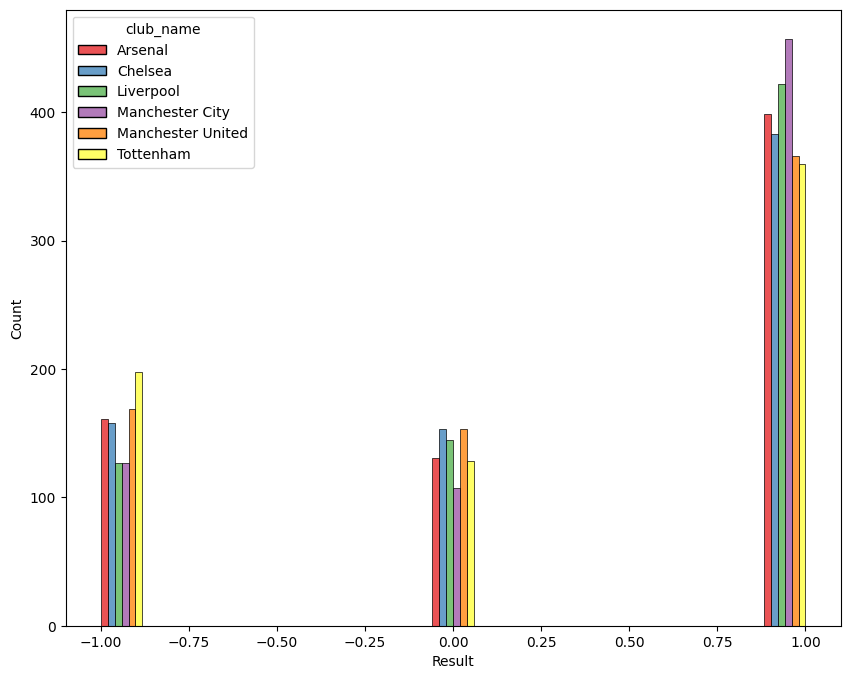
\includegraphics[keepaspectratio]{premier_league_files/figure-pdf/cell-18-output-1.png}}

\begin{Shaded}
\begin{Highlighting}[]
\ImportTok{from}\NormalTok{ sklearn.preprocessing }\ImportTok{import}\NormalTok{ LabelEncoder}

\CommentTok{\# Los 6 equipos principales}
\NormalTok{main\_teams }\OperatorTok{=}\NormalTok{ [}
    \StringTok{"Liverpool"}\NormalTok{, }\StringTok{"Chelsea"}\NormalTok{, }\StringTok{"Arsenal"}\NormalTok{,}
    \StringTok{"Manchester City"}\NormalTok{, }\StringTok{"Manchester United"}\NormalTok{, }\StringTok{"Tottenham"}
\NormalTok{]}

\CommentTok{\# Unir todos los valores de ambas columnas}
\NormalTok{all\_teams }\OperatorTok{=}\NormalTok{ pd.concat([df\_final[}\StringTok{\textquotesingle{}club\_name\textquotesingle{}}\NormalTok{], df\_final[}\StringTok{\textquotesingle{}Opponent\textquotesingle{}}\NormalTok{]]).unique()}

\CommentTok{\# Crear el encoder y ajustarlo}
\NormalTok{encoder }\OperatorTok{=}\NormalTok{ LabelEncoder()}
\NormalTok{encoder.fit(all\_teams)}

\CommentTok{\# Aplicar encoding a las columnas}
\NormalTok{df\_final[}\StringTok{\textquotesingle{}club\_name\_enc\textquotesingle{}}\NormalTok{] }\OperatorTok{=}\NormalTok{ encoder.transform(df\_final[}\StringTok{\textquotesingle{}club\_name\textquotesingle{}}\NormalTok{])}
\NormalTok{df\_final[}\StringTok{\textquotesingle{}opponent\_enc\textquotesingle{}}\NormalTok{]  }\OperatorTok{=}\NormalTok{ encoder.transform(df\_final[}\StringTok{\textquotesingle{}Opponent\textquotesingle{}}\NormalTok{])}
\NormalTok{df\_final }\OperatorTok{=}\NormalTok{ df\_final.drop(columns}\OperatorTok{=}\NormalTok{[}\StringTok{\textquotesingle{}club\_name\textquotesingle{}}\NormalTok{,}\StringTok{\textquotesingle{}Opponent\textquotesingle{}}\NormalTok{])}

\CommentTok{\# Crear diccionario con los 6 equipos principales y su número}
\NormalTok{main\_team\_labels }\OperatorTok{=}\NormalTok{ \{team: encoder.transform([team])[}\DecValTok{0}\NormalTok{] }\ControlFlowTok{for}\NormalTok{ team }\KeywordTok{in}\NormalTok{ main\_teams\}}

\BuiltInTok{print}\NormalTok{(}\StringTok{"📌 Labels de los equipos principales:"}\NormalTok{)}
\BuiltInTok{print}\NormalTok{(main\_team\_labels)}
\end{Highlighting}
\end{Shaded}

\begin{verbatim}
📌 Labels de los equipos principales:
{'Liverpool': np.int64(219), 'Chelsea': np.int64(100), 'Arsenal': np.int64(18), 'Manchester City': np.int64(237), 'Manchester United': np.int64(239), 'Tottenham': np.int64(418)}
\end{verbatim}

\begin{Shaded}
\begin{Highlighting}[]
\NormalTok{df\_final.head(}\DecValTok{5}\NormalTok{)}
\end{Highlighting}
\end{Shaded}

\begin{longtable}[]{@{}lllllllllllllllllllllllllllllllllllllll@{}}
\toprule\noalign{}
& Is\_Home & Result & Goals & Opponent\_Goals & Possession & Shots &
Shots\_On\_Target & Passes\_Completed & Pass\_Accuracy & Corners &
Crosses & Fouls & Offsides & Opponent\_Possession & Opponent\_Shots &
Opponent\_Shots\_On\_Target & Opponent\_Passes\_Completed &
Opponent\_Pass\_Accuracy & Opponent\_Corners & Opponent\_Crosses &
Opponent\_Fouls & Opponent\_Offsides & Shot\_Efficiency & Season & Month
& Day\_of\_Week & Last5\_Avg\_Goals & Last5\_Win\_Rate & Date\_day &
Date\_month & Date\_year & Date\_weekday & Date\_quarter & Date\_hour &
Date\_minute & Date\_second & club\_name\_enc & opponent\_enc \\
\midrule\noalign{}
\endhead
\bottomrule\noalign{}
\endlastfoot
0 & 1 & -1 & 1 & 2 & 55 & 12 & 5 & 425 & 80 & 4 & 2 & 12 & 2 & 45 & 12 &
6 & 399 & 81 & 5 & 3 & 15 & 2 & 0.416667 & 2013 & 8 & 7 & 1.000000 &
0.00 & 4 & 8 & 2013 & 6 & 3 & 18 & 20 & 0 & 18 & 159 \\
1 & 1 & -1 & 1 & 3 & 64 & 15 & 4 & 457 & 87 & 4 & 4 & 15 & 3 & 36 & 10 &
5 & 216 & 71 & 3 & 2 & 19 & 1 & 0.266667 & 2013 & 8 & 6 & 1.000000 &
0.00 & 17 & 8 & 2013 & 5 & 3 & 17 & 0 & 0 & 18 & 23 \\
2 & 0 & 1 & 3 & 0 & 60 & 13 & 7 & 451 & 84 & 6 & 2 & 14 & 0 & 40 & 6 & 2
& 350 & 79 & 5 & 2 & 15 & 1 & 0.538462 & 2013 & 8 & 3 & 1.666667 & 0.33
& 21 & 8 & 2013 & 2 & 3 & 21 & 45 & 0 & 18 & 146 \\
3 & 0 & 1 & 3 & 1 & 54 & 19 & 9 & 496 & 87 & 8 & 9 & 9 & 0 & 46 & 16 & 7
& 421 & 87 & 1 & 1 & 10 & 3 & 0.473684 & 2013 & 8 & 6 & 2.000000 & 0.50
& 24 & 8 & 2013 & 5 & 3 & 14 & 45 & 0 & 18 & 156 \\
4 & 1 & 1 & 2 & 0 & 65 & 14 & 6 & 460 & 86 & 2 & 4 & 16 & 2 & 35 & 6 & 4
& 350 & 79 & 3 & 4 & 16 & 1 & 0.428571 & 2013 & 8 & 2 & 2.000000 & 0.60
& 27 & 8 & 2013 & 1 & 3 & 21 & 45 & 0 & 18 & 147 \\
\end{longtable}




\end{document}
